% Netzwerkanltung für die Studentenstadt Freimann
% Tex initially created by Maximilian Engelhardt <maximilian.engelhardt@stusta.mhn.de>

%\documentclass[a4paper,12pt,draft]{scrartcl}
\documentclass[a4paper,12pt]{scrartcl}

\usepackage[utf8]{inputenc}
\usepackage{ngerman}
\usepackage{eurosym}
\usepackage{tabularx}
\usepackage[pdftex,final]{graphicx}
\usepackage{wrapfig}
\usepackage[top=1.5cm,bottom=2.5cm,left=1.5cm,right=1.5cm]{geometry}
%\usepackage[margin=2cm]{geometry}
\usepackage{hyperref}


\title{Wohnanlage Studentenstadt Freimann:\\
       Anleitung zum Einrichten des Internetzugangs}
%\date{\today}

\begin{document}

\maketitle

\begin{figure}[t!]
   \centering
   \vspace{-20pt}
   
\includegraphics[width=0.8\textwidth,keepaspectratio]{Bilder/StuStaNet_Logo}
   \vspace{-40pt}
\end{figure}

\section*{Allgemeine Informationen zum Netzwerkanschluss}

Dies ist eine Beschreibung, wie Sie ihren Computer an das Netzwerk der Studentenstadt anschließen. Lesen Sie vorher die Benutzerordnung gründlich durch, die Sie mit ihrem Mietvertrag erhalten haben.
\\
\\
Sie benötigen einen Computer mit LAN-Kabelanschluss, und ein LAN-Kabel zum Anschluss des Computers an der im Zimmer angebrachten Netzwerkdose. Diese Kabel können im Fachhandel oder auch beim StuStaNet e.V. während der Sprechstunde (siehe weiter unten) erworben werden.
\\
\\
Jeder, der seinen Computer an das Netzwerk der Studentenstadt anschließt, ist dafür verantwortlich, dass dadurch keine anderen Rechner im Netzwerk gefährdet werden. Dazu gehört seinen Rechner vor Viren oder anderer Schadsoftware zu schützen.
Der Stustanet~e.V. betreibt eine Schadsoftwareerkennung, die Anschlüsse bei Auffälligkeiten aufgrund von Virenbefall vorübergehend sperrt.
\\
\begin{bfseries}
	\\Bei wiederholter Virendiagnose wird der entsprechende Anschluss dauerhaft gesperrt.
\end{bfseries}




%\pagebreak

\section*{Mitgliedschaft StuStaNet e.V.}
Es gibt zwei Möglichkeiten im Internet zu surfen. Die Standard-Variante ist der Zugang über den Proxyserver. Allerdings muss dieser bei jeder Applikation eingestellt werden, falls dies unterstützt wird. Die andere Möglichkeit ist über unser NAT-Gateway. Dies und einige andere Dienste\footnote{http://wiki.stusta.de/Dienste} stehen für Mitglieder des StuStaNet e.V. zur Verfügung. Die Konfiguration des Proxys kann dann entfallen.
\\
\\
Für die Mitgliedschaft fällt eine \textbf{einmalige} Gebühr von \EUR{20} an. Um Mitglied zu werden, registrieren Sie sich bitte vorab unter \mbox{\url{https://reg.stusta.de}} und kommen Sie zu einer unserer Sprechstunden im Blauen Haus, Zimmer 028. 
\\
Die Sprechstunden finden meist Donnerstags 19:00-19:30 Uhr statt. Zu Beginn des Semesters zusätzlich Montags 19:00-19:30 Uhr.
\\
Die genauen Zeiten sind verfügbar unter \mbox{\url{http://sprechstunden.stusta.de}}.

\section*{Netzwerkkonfiguration}
\subsection*{Überblick}

Das Einrichten der Internetanbindung besteht aus folgenden Teilen:
\begin{itemize}
	\item Anschluss an die Netzwerkbuchse
	\item Konfiguration der Netzwerkeinstellungen im Betriebssystem
	\item Eintragen des Proxyservers bzw. -skripts im Browser
\end{itemize}
Verwenden Sie ausschließlich die \emph{linke} Netzwerkbuchse. 
 


\subsubsection*{WLAN}
In der StuSta gibt es kein zentrales WLAN, allerdings kann jeder selbst einen Access Point betreiben. In den Einstellungen des Routers/AP muss eine der Zimmer-IPs, sowie Gateway, Subnetzmakse und DNS eingestellt werden.
\\
\\
Der StuStaNet e.V. verkauft für die StuSta passend vorkonfigurierte Geräte in der Sprechstunde (nur an Mitglieder und nur solange der Vorrat reicht).





\subsection*{Konfiguration der Netzwerkeinstellungen}

Pro Anschluss stehen 8 IP-Adressen zur Verfügung. Der jeweilige Adressbereich ist auf der Netzwerkdose vermerkt oder auf dem Internetkonfigurationsblatt zu finden, das Sie mit Ihrem Mietvertrag von der Hausverwaltung erhalten haben. Sollten Sie dieses Blatt nicht mehr finden, wenden Sie sich bitte an die Hausverwaltung \footnote{Christoph-Probst-Straße 10, Studentenstadt Freimann}.




\begin{center}
  \begin{tabularx}{\linewidth}{|lXp{.2\linewidth}|}
    \hline
    Einstellung & Wert & Beispiel \\
    \hline \hline
    IP-Adresse & \nolinkurl{10.150.xxx.yyy} - \nolinkurl{10.150.xxx.zzz}, \newline 8 Adressen stehen zur Auswahl\footnote{Man findet sie auf der Netzwerkdose im Zimmer oder auf dem IP-Zettel, erhältlich bei der Hausverwaltung.} & \nolinkurl{10.150.243.16} – \nolinkurl{10.150.243.23} \\
    \hline
    Subnetzmaske & \nolinkurl{255.255.255.0} & \\
    \hline
    Standardgateway & \nolinkurl{10.150.xxx.254} \newline (Die ersten drei Blöcke wie IP-Adresse, der vierte Block \nolinkurl{254}) & \nolinkurl{10.150.243.254} \\
    \hline
    DNS-Server (Nameserver) & \nolinkurl{10.150.127.2} \newline \nolinkurl{10.150.125.2} & \\
    \hline
    DNS-Suffix (Domainname) & \nolinkurl{stusta.mhn.de} & \\
    \hline
    Proxyskript & \multicolumn{2}{l|}{\nolinkurl{http://wpad.stusta.mhn.de/proxy.pac}} \\
    \hline
    Proxyserver (manuell) & \multicolumn{2}{l|}{\nolinkurl{http://proxy.stusta.mhn.de:3128}} \\
    \hline
  \end{tabularx}
\end{center}
Bei Nicht-Mitgliedschaft muss entweder das Proxyskript verwendet oder manuell der Proxyserver eingestellt werden. Die Verwendung des \emph{Proxyskripts} wird stark empfohlen!

\newpage
\enlargethispage{20pt}






\begin{figure}[h]
	\raggedleft
	\vspace{-20pt}
	
\includegraphics[height=1cm,keepaspectratio]{Bilder/Windows_logo}
	\vspace{-30pt}
\end{figure}

\section*{Schritt für Schritt Anleitung Windows}
\subsection*{Windows XP}
Es wird von dem Gebrauch von XP abgeraten, da Windows den Support eingestellt hat und dieses System daher nicht mehr ausreichend geschützt ist. 

\subsection*{Windows Vista/7}
\begin{enumerate}
    \item Öffnen Sie die \emph{Systemsteuerung} durch Klick auf \emph{Start} $\rightarrow$ \emph{Systemsteuerung}.
    \item Wählen Sie unter \emph{Netzwerk und Internet} den Punkt \emph{Netzwerkstatus und -aufgaben} anzeigen.
    \item Nach Klick auf \emph{Netzwerkverbindungen} verwalten wählen Sie im darauffolgenden Fenster durch einen Rechtsklick auf LAN-Verbindung deren Eigenschaften aus.
\end{enumerate}
$\rightarrow$ Weiter bei Punkt 5.
      \begin{figure}[h!]
	\centering
        \vspace{-5pt}
        \begin{minipage}[c]{0.45\linewidth}
          \centering
          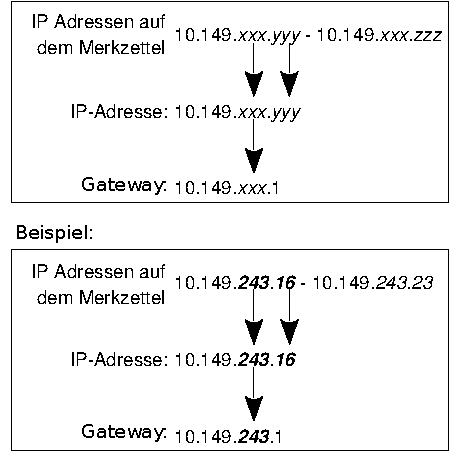
\includegraphics[width=\linewidth,keepaspectratio]{Bilder/IP_Gerneric}
        \end{minipage}
        \begin{minipage}[c]{0.48\linewidth}
          \centering
          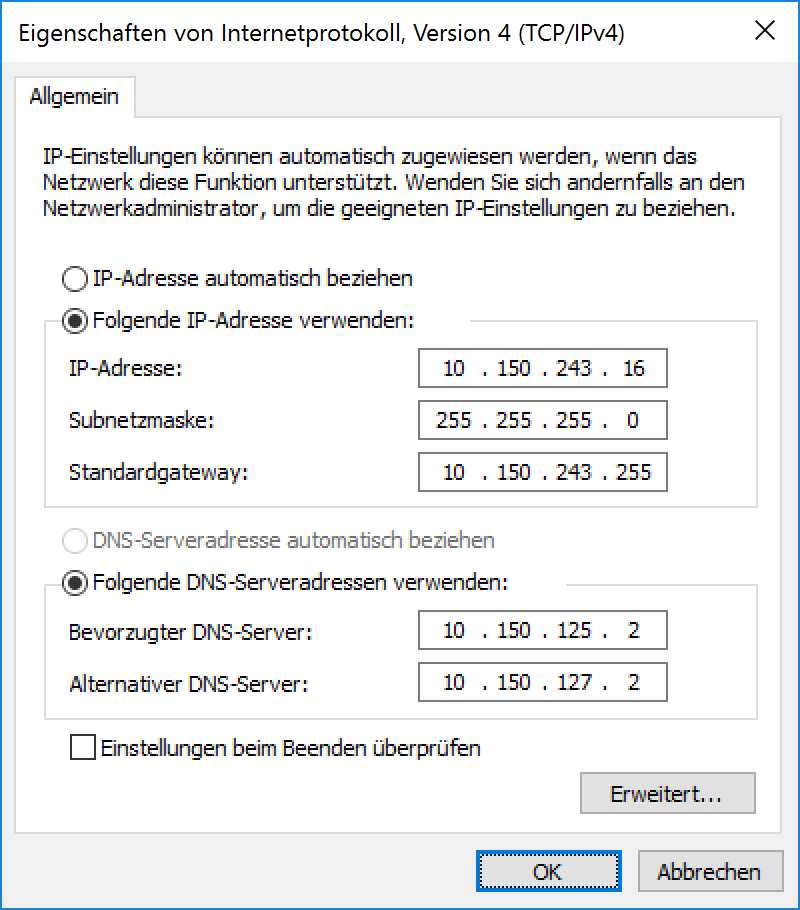
\includegraphics[width=\linewidth,keepaspectratio]{Bilder/IP_Windows}
          \caption{Beispielhafte Netzwerkeinstellungen unter Windows Vista}
        \end{minipage}
      \vspace{-20pt}
      \end{figure}
\subsection*{Windows 8}
\begin{enumerate}
	\item Öffnen Sie die Systemsteuerung, in dem Sie die Windows-Taste drücken, \glqq Systemsteuerung\grqq  \ eingeben und ENTER drücken
	\item Wählen Sie unter Netzwerk und Internet den Punkt Netzwerkstatus und -aufgaben anzeigen.
    \item Nach Klick auf Netzwerkverbindungen verwalten wählen Sie im darauffolgenden Fenster durch einen Rechtsklick auf LAN-Verbindung deren Eigenschaften aus.
\end{enumerate}
$\rightarrow$ Weiter bei Punkt 5.

\subsection*{Windows 10}
\begin{enumerate}
	\item Klicken Sie auf das Windowssymbol in der unteren linken Ecke und anschließend auf \emph{Einstellungen}
	\item Klicken Sie auf \textit{Netzwerk und Freigabecenter} und wählen Sie unter \textit{Verwandte Einstellungen} den Punkt \textit{Adapteroptionen ändern}. Sollten Sie diesen Punkt nicht finden können Sie auch in der Suchzeile rechts oben nach \glqq Adapteroptionen ändern\grqq suchen.
    \item Ihnen sollten nun mehrere Netzwerkverbindungen aufgelistet sein. Klicken Sie mit der \textbf{rechten} Maustaste auf \textit{Local Area Connection} und klicken Sie dann auf \textit{Eigenschaften}.
\end{enumerate}
$\rightarrow$ Weiter bei Punkt 5.

\subsection*{Windows Vista/7/8/10}
\begin{enumerate}
    \setcounter{enumi}{4}
    \item Markieren Sie den Eintrag \textit{Internetprotokoll Version 4 (TCP/IPv4)} (Windows Vista/7/8/10) bzw. Internetprotokoll  (TCP/IP) (Windows XP) und klicken Sie danach auf Eigenschaften.
    \item Jetzt geben Sie IP-Adresse, Subnetzmaske, Standardgateway und DNS Server ein. Die Adressen der DNS-Server lauten \textbf{10.150.127.2} und \textbf{10.150.125.2}, die Subnetzmaske \textbf{255.255.255.0}. Ihre jeweilige IP-Adresse steht auf einem Aufkleber auf Ihrer Anschlussbuchse bzw. auf dem Zettel, den Sie mit Ihrem Mietvertrag erhalten haben. Sollten Sie keinen Zettel mit Netzwerkdaten bekommen haben und der Aufkleber auf der Anschlussbuchse unlesbar sein, wenden Sie sich bitte an die Hausverwaltung.
    \item Klicken Sie auf Erweitert und wählen im folgenden Dialog den Reiter DNS aus. Tragen Sie im Feld DNS-Suffix für diese Verbindung \textbf{stusta.mhn.de} ein.
    \item Bestätigen mit OK.
\end{enumerate}
$\rightarrow$ Weiter bei den Browsereinstellungen.



\pagebreak

\begin{figure}[t!]
	\raggedleft
	\vspace{-20pt}
	
\includegraphics[height=1cm,keepaspectratio]{Bilder/Ubuntu_logo}
	\vspace{-30pt}
\end{figure}



\section*{Schritt für Schritt Anleitung Ubuntu}

\begin{enumerate}
	\item Öffnen Sie die Netzwerkkonfiguration durch Klick auf \emph{System} $\rightarrow$ \emph{Einstellungen} $\rightarrow$ \emph{Netzwerkkonfiguration}.
	\item Markieren Sie nun im Reiter Kabelgebunden den entsprechenden Eintrag Ihrer Netzwerkkarte (im Normalfall \emph{eth0}) und klicken Sie auf den Button \emph{Bearbeiten}.
	\item Gehen Sie zum Reiter \emph{IPv4-Einstellungen} und setzen Sie Methode auf \emph{Manuell}.
	\item Unter \emph{Adressen} klicken Sie auf den Button \emph{Hinzufügen}.
	\begin{figure}[h!]
		\centering
		\begin{minipage}[c]{0.45\linewidth}
			\centering
			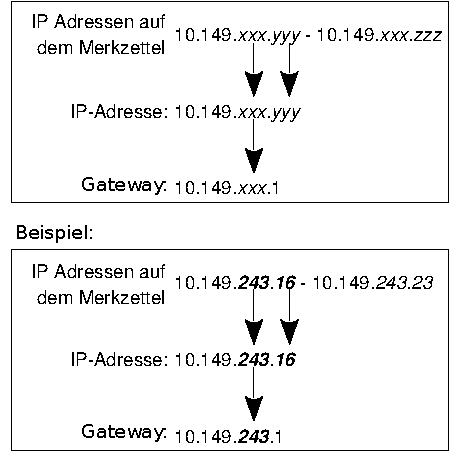
\includegraphics[width=\linewidth,keepaspectratio]{Bilder/IP_Gerneric}
		\end{minipage}
		\begin{minipage}[c]{0.5\linewidth}
			\centering
			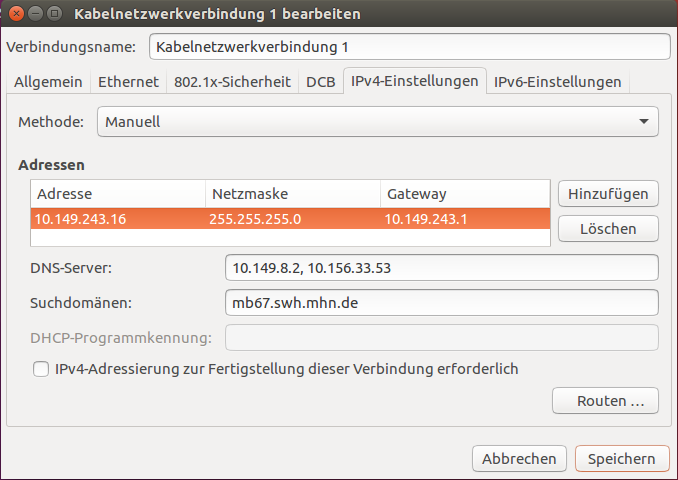
\includegraphics[width=0.9\linewidth,keepaspectratio]{Bilder/IP_Ubuntu}
			\caption{Beispielhafte Netzwerkeinstellungen unter Ubuntu Linux}
			\vspace{-15pt}
		\end{minipage}
	\end{figure}
	\item Jetzt geben Sie IP-Adresse, Subnetzmaske, Gateway, DNS und Suchdomäne ein. Die Adressen der DNS-Server lauten \textbf{10.150.127.2} und \textbf{10.150.125.2}, die Suchdomäne \textbf{stusta.mhn.de} und die Netzmaske \textbf{255.255.255.0}. Ihre jeweilige IP-Adresse steht auf einem Aufkleber auf Ihrer Anschlussbuchse bzw. auf dem Zettel, den Sie mit Ihrem Mietvertrag erhalten haben. Sollten Sie einen neuen Zettel benötigen, wenden Sie sich bitte an die Hausverwaltung. Bestätigen Sie mit \emph{OK} und schließen Sie das Fenster für die Netzwerkeinstellungen.
\end{enumerate}

\subsection*{Proxy global einstellen} Unter Ubuntu haben Sie die Möglichkeit den Proxy global zu definieren, sodass dieser nicht extra für jedes Programm eingetragen werden.
\begin{enumerate}
	\item Öffnen Sie die Netzwerk-Proxy-Einstellungen durch Klick auf \emph{System} $\rightarrow$ \emph{Einstellungen} $\rightarrow$ \emph{Netzwerk-Proxy}.
	\item Hier markieren Sie ganz unten die Option \emph{Automatische Proxy-Konfiguration} und tragen bei URL für Auto-Konfiguration: \url{http://wpad.stusta.mhn.de/proxy.pac} ein. Schließen Sie das Fenster. 
\end{enumerate}



\newpage
\enlargethispage{20pt}



\begin{figure}[t!]
	\raggedleft
	\vspace{-20pt}
	
\includegraphics[height=1cm,keepaspectratio]{Bilder/OSXLeopard}
	\vspace{-30pt}
\end{figure}
\section*{Schritt für Schritt Anleitung Mac OS X}
\begin{enumerate}
    \item Öffnen Sie die Netzwerkkonfiguration durch Klick auf \emph{Apfel} (oben links) und wählen dann \emph{Systemeinstellungen} $\rightarrow$ \emph{Netzwerk} aus.
    \item Markieren Sie nun das Netzwerkgerät \emph{Ethernet}.
    \item Setzen Sie das Feld \emph{IPv4 Konfigurieren} auf \emph{Manuell}.
    \item Jetzt geben Sie \textbf{IP-Adresse, Teilnetzmaske, Gateway, DNS-Server} und \textbf{Such-Domains} ein. Die Adressen der DNS-Server lauten \textbf{10.150.127.2} und \textbf{10.150.125.2}, die Such-Domains \textbf{stusta.mhn.de} und die Teilnetzmaske \textbf{255.255.255.0}. Ihre jeweilige IP-Adresse steht auf einem Aufkleber auf Ihrer Anschlussbuchse bzw. auf dem Internetkonfigurationsblatt, das Sie mit Ihrem Mietvertrag erhalten haben. Sollten Sie dieses Blatt nicht mehr finden, wenden Sie sich bitte an die Hausverwaltung \footnote{Christoph-Probst Straße 10, Studentenstadt Freimann}. Bestätigen Sie mit \emph{Anwenden}.
      \begin{figure}[h!]
      \centering
%      \vspace{-5pt}
        \begin{minipage}[c]{0.38\linewidth}
          \centering
          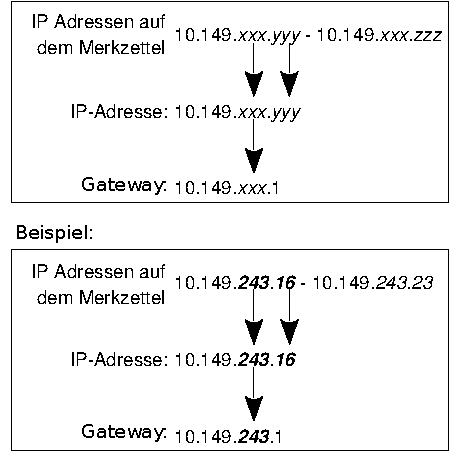
\includegraphics[width=\linewidth,keepaspectratio]{Bilder/IP_Gerneric}
        \end{minipage}
        \begin{minipage}[c]{0.60\linewidth}
          \centering
          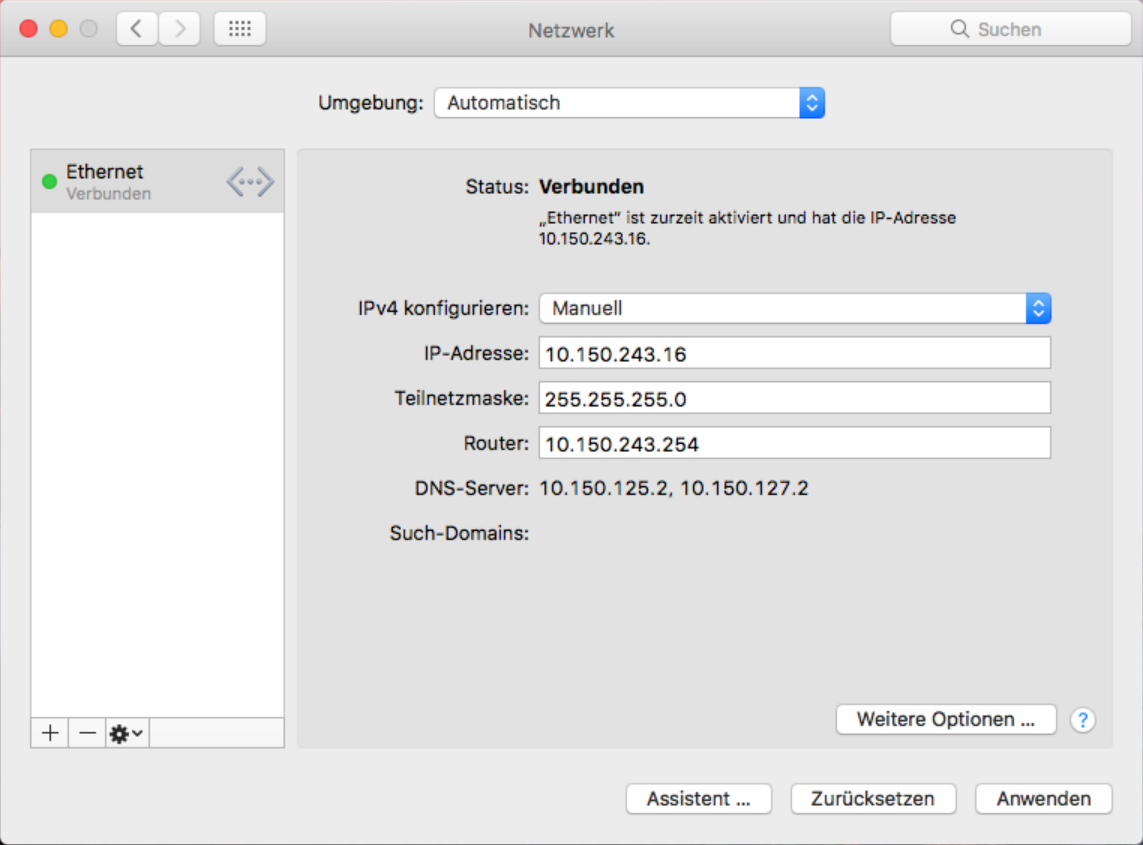
\includegraphics[width=0.9\linewidth,keepaspectratio]{Bilder/IP_MAC}
          \caption{Beispielhafte Netzwerkeinstellungen unter Mac OS~X}
        \end{minipage}
      \vspace{-20pt}
      \end{figure}
\end{enumerate}
\vspace{-15pt}
\subsection*{Proxy global einstellen}
Unter Mac OS X haben Sie die Möglichkeit den Proxy global zu definieren, sodass dieser nicht extra für jedes Programm eingetragen werden muss. Firefox benötigt allerdings trotzdem eine gesonderte Einstellungen (siehe Browsereinstellungen). %noch aktuelle info??

%\begin{wrapfigure}{r}{0.4\textwidth}
%  \vspace{-20pt}
%  \begin{center}
%    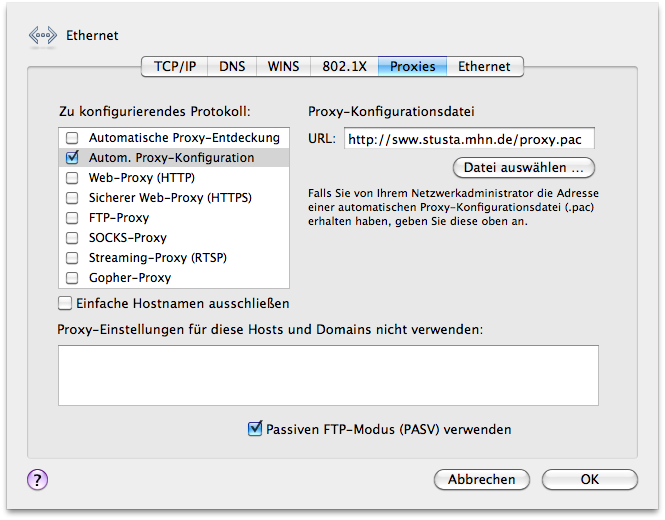
\includegraphics[width=0.48\textwidth,keepaspectratio]{Bilder/Proxy_MAC}
%  \end{center}
%  \vspace{-20pt}
%  \caption{Beispielhafte Proxyeinstellungen unter Mac OS~X}
%  \vspace{-10pt}
%\end{wrapfigure}
\begin{enumerate}%WTF 1. punkt???
    \item Öffnen Sie mit dem Button \emph{Weitere Optionen...} im voherigen Dialog die Detaileinstellungen und wechseln sie auf die Registerkarte \emph{Proxies}
    \item Setzen sie bei Zu konfigurierendes Protokoll vor Autom. Proxy-Konfiguration einen Hacken und tragen rechts bei URL \url{http://wpad.stusta.mhn.de/proxy.pac} ein. Schließen Sie die Detaileinstellungen mit OK und bestätigen Sie erneut mit Anwenden. Sie können die Netzwerkeinstellungen jetzt schließen.
\end{enumerate}
$\rightarrow$ Der Internetzugang ist jetzt fertig konfiguriert.

\newpage

\section*{Proxy-Konfiguration im Browser (nur Nicht-Mitglieder)}
\label{Proxy}

\begin{wrapfigure}{r}{0.5\textwidth}
	\vspace{-40pt}
	\begin{center}
		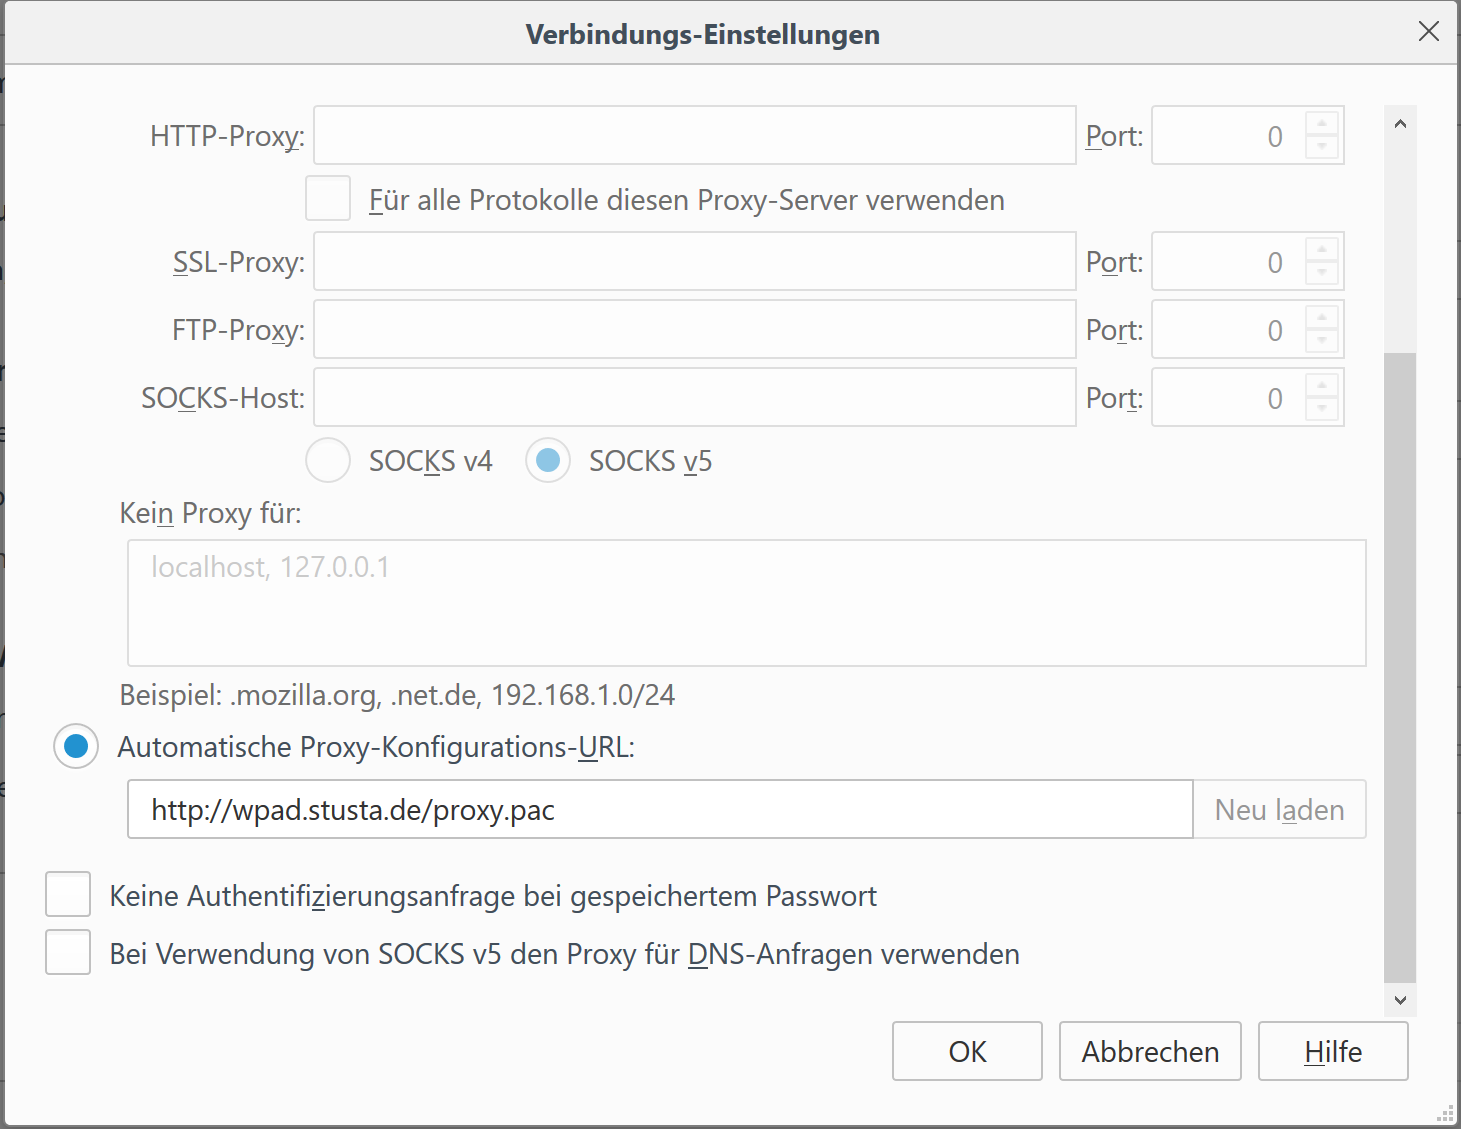
\includegraphics[width=0.5\textwidth,keepaspectratio]{Bilder/Proxy_Firefox}
	\end{center}
	%  \vspace{-20pt}
	\caption{Eintragen des Proxyskripts in Mozilla Firefox}
	%  \vspace{-10pt}
\end{wrapfigure}

\subsection*{
\includegraphics[height=1.2cm,keepaspectratio]{Bilder/Firefox_35_logo} Mozilla Firefox}
\begin{enumerate}
	\item Klicken Sie auf die 3 übereinanderliegenden Striche in der rechten oberen Ecke, wählen Sie danach \emph{Einstellungen}
	\item Wählen Sie im linken Menü den Punkt \emph{Erweitert}
	\item Wählen Sie in der oberen Leiste den Punkt \emph{Netzwerk}
	\item Klicken Sie rechts neben dem ersten Unterpunkt \emph{Verbindung} auf \emph{Einstellungen}
	\item Markieren Sie den untersten Punkt und tragen Sie als Automatische Proxy-Konfigurations-URL: \\ \url{http://wpad.stusta.mhn.de/proxy.pac} ein.
	\item Bestätigen Sie mit OK und schließen Sie die restlichen Fenster.\\
	\\
	\\
\end{enumerate}


\begin{wrapfigure}{r}{0.5\textwidth}
	%  \vspace{-20pt}
	\begin{center}
		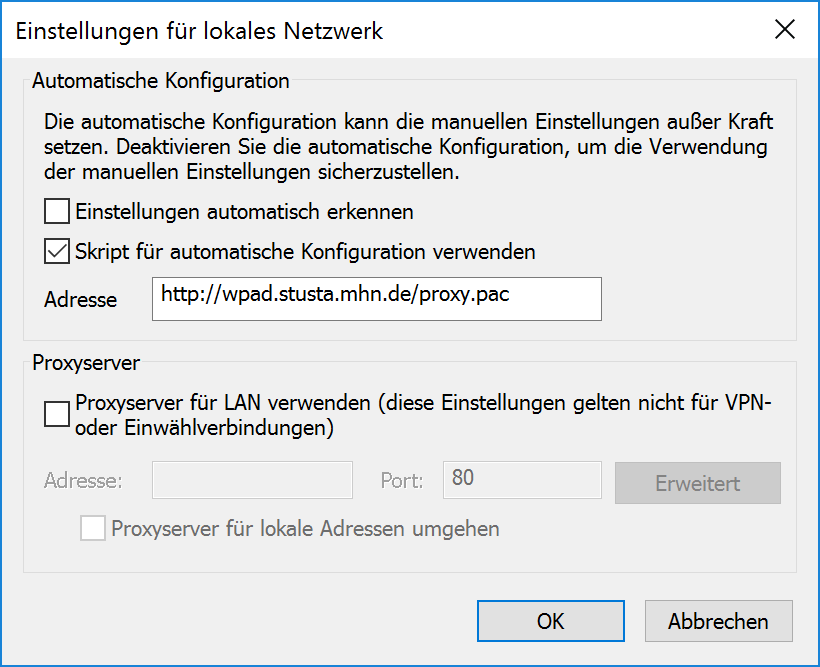
\includegraphics[width=0.5\textwidth,keepaspectratio]{Bilder/Proxy_IE}
	\end{center}
	%  \vspace{-20pt}
	\caption{Eintragen des Proxyskripts im Internet Explorer}
	%  \vspace{-10pt}
\end{wrapfigure}

\subsection*{
\includegraphics[height=1.2cm,keepaspectratio]{Bilder/Internet_Explorer_7_Logo} Internet Explorer}
\begin{enumerate}
	\item Internet Explorer starten.
	\item Wählen Sie im Untermenü Extras den Punkt Internetoptionen.
	\item Im Reiter Verbindungen auf den Button LAN-Ein\-stellungen klicken.
	\item Setzen Sie bei Automatisches Konfigurationsskript verwenden einen Haken und tragen Sie bei der Adresse \\ \url{http://wpad.stusta.mhn.de/proxy.pac} ein.
	\item Bestätigen Sie mit OK und schließen Sie die restlichen Fenster.
\end{enumerate}
$\rightarrow$ Der Internetzugang ist nun fertig konfiguriert.


\newpage
\begin{wrapfigure}{r}{0.5\textwidth}
	\vspace{-40pt}
	\begin{center}
		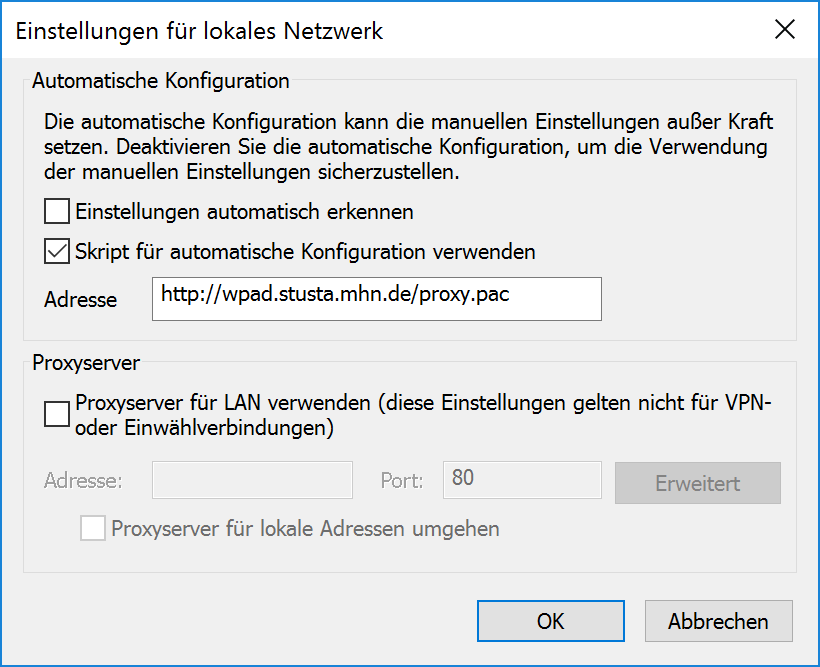
\includegraphics[width=0.5\textwidth,keepaspectratio]{Bilder/Proxy_IE.png}
	\end{center}
	%  \vspace{-20pt}
	\caption{Eintragen des Proxyskripts in Google Chrome}
	%  \vspace{-10pt}
\end{wrapfigure}
\subsection*{
\includegraphics[height=1.2cm,keepaspectratio]{Bilder/Chrome_2011_logo} Google Chrome}
\begin{enumerate}
	\item Chrome starten
	\item Klicken Sie auf die 3 übereinanderliegenden Striche in der rechten oberen Ecke, wählen Sie danach \emph{Einstellungen}
	\item Wählen Sie den Punkt \emph{Erweiterte Einstellungen anzeigen}
	\item Klicken Sie auf \emph{Proxyeinstellungen ändern...}
	\item Im Reiter Verbindungen auf den Button \emph{LAN-Ein\-stellungen} klicken.
	\item Setzen Sie bei Automatisches Konfigurationsskript verwenden einen Haken und tragen Sie bei der Adresse \\ \url{http://wpad.stusta.mhn.de/proxy.pac} ein.
	\item Bestätigen Sie mit OK und schließen Sie die restlichen Fenster.
	\\
	\\
\end{enumerate}


\begin{wrapfigure}{r}{0.5\textwidth}
	%  \vspace{-20pt}
	\begin{center}
		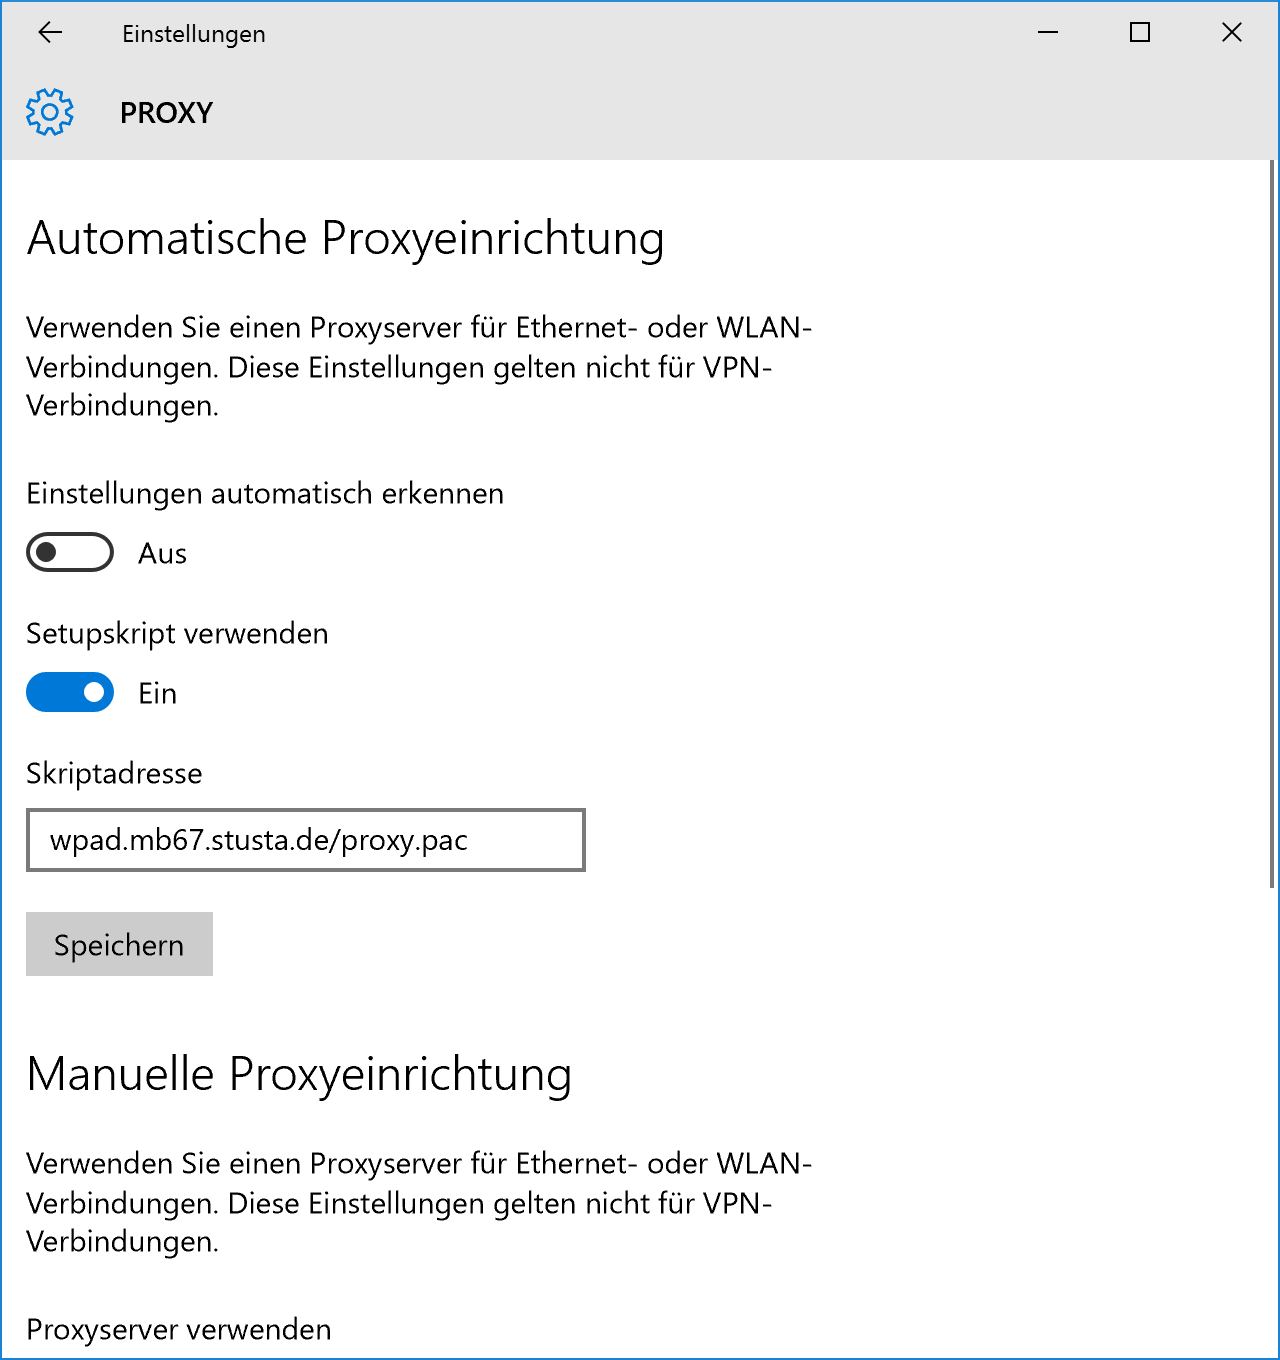
\includegraphics[width=0.5\textwidth,keepaspectratio]{Bilder/Proxy_Edge}
	\end{center}
	%  \vspace{-20pt}
	\caption{Eintragen des Proxyskripts in Microsoft Edge}
	%  \vspace{-10pt}
\end{wrapfigure}

\subsection*{
\includegraphics[height=1.2cm,keepaspectratio]{Bilder/Mcrosoft_Edge_logo} Microsoft Edge}
\begin{enumerate}
	\item Microsoft Edge starten.
	\item Klicken Sie auf die 3 übereinanderliegenden Striche in der rechten oberen Ecke, wählen Sie danach \emph{Einstellungen}
	\item Wählen Sie den Punkt \emph{Erweiterte Einstellungen anzeigen}
	\item Klicken Sie auf \emph{Proxyeinstellungen öffnen}
	\item Deaktivieren Sie die Option \emph{Einstellungen automatisch erkennen}
	\item Wählen Sie \emph{Setupskript verwenden} und tragen Sie bei der Adresse \\ \url{http://wpad.stusta.mhn.de/proxy.pac} ein.
	\item Klicken Sie auf speichern und schließen Sie die geöffneten 
	Fenster.
\end{enumerate}
$\rightarrow$ Der Internetzugang ist nun fertig konfiguriert.

%\newpage
%\begin{wrapfigure}{r}{0.5\textwidth}
%%  \vspace{-20pt}
%  \begin{center}
%    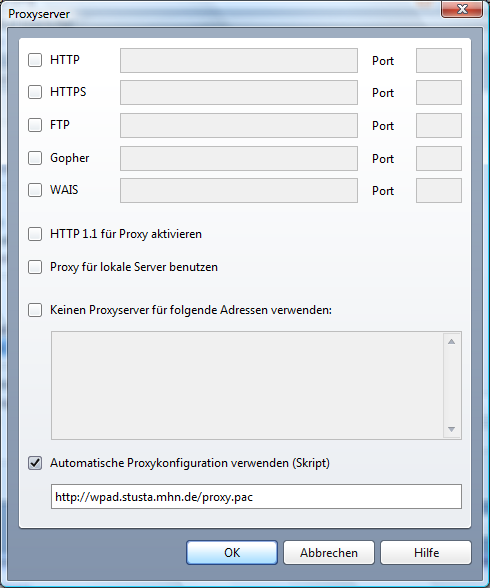
\includegraphics[width=0.5\textwidth,keepaspectratio]{Bilder/Proxy_Opera}
%  \end{center}
%%  \vspace{-20pt}
%  \caption{Eintragen des Proxyskripts im Opera}
%%  \vspace{-10pt}
%\end{wrapfigure}
%
%\subsection*{
\includegraphics[height=1.2cm,keepaspectratio]{Bilder/Opera_O} Opera}
%\begin{enumerate}
%    \item Opera starten.
%    \item Wählen Sie im Untermenü Extras den Punkt Einstellungen...
%    \item Wählen Sie im Reiter Erweitert auf der linken Seite die Kategorie Netzwerk und dann klicken Sie auf den Button Proxy.
%    \item Setzen Sie bei Automatische Proxykonfiguration verwenden (Skript) einen Haken und tragen Sie \\ \url{http://wpad.mb67.stusta.mhn.de/proxy.pac} ein.
%    \item Schließen Sie beide Fenster mit OK.
%\end{enumerate}
%$\rightarrow$ Der Internetzugang ist nun fertig konfiguriert.


\end{document}
